\documentclass{article}

% content/resources/templates/preamble.tex
\usepackage[margin=0.6in]{geometry}
\author{Milav Dabgar}
\usepackage{amsmath,amssymb,amsthm}
\usepackage{booktabs}
\usepackage{multirow}
\usepackage{xcolor}
\usepackage{tcolorbox}
\tcbuselibrary{breakable,skins}
\usepackage[colorlinks=true,linkcolor=blue]{hyperref}
\usepackage{titlesec}
\usepackage{enumitem}
\usepackage{tikz}
\usepackage{pgfplots}
\usepackage{circuitikz}
\usepackage[version=4]{mhchem}
\usepackage{longtable}
\usepackage{array}
\usepackage{float}
\usepackage{caption}
\usepackage{listings}

\lstset{
  basicstyle=\small\ttfamily,
  breaklines=true,
  breakatwhitespace=false,
  postbreak=\mbox{\textcolor{red}{$\hookrightarrow$}\space},
  float=false,
  numbers=left,
  numberstyle=\tiny\color{gray},
  numbersep=10pt,
  xleftmargin=2em,
  keywordstyle=\color{blue},
  commentstyle=\color{green!60!black},
  stringstyle=\color{purple},
  backgroundcolor=\color{gray!5},
  showstringspaces=false,
  tabsize=2,
  captionpos=b,
  keepspaces=true,
  columns=flexible
}

\pgfplotsset{compat=1.18}
\usetikzlibrary{shapes,arrows,positioning,calc,patterns,decorations.pathmorphing,decorations.markings,arrows.meta}

% Color scheme
\definecolor{headcolor}{RGB}{0,102,204}
\definecolor{keycolor}{RGB}{220,20,60}
\definecolor{solutioncolor}{RGB}{34,139,34}
\definecolor{mnemoniccolor}{RGB}{148,0,211}
\definecolor{codecolor}{RGB}{0,0,100}

% Spacing
\setlength{\parskip}{3pt}
\setlist[itemize]{nosep}
\setlist[enumerate]{nosep}

% Title formatting
\titleformat{\section}{\Large\bfseries\color{headcolor}}{\thesection}{1em}{}
\titleformat{\subsection}{\large\bfseries\color{headcolor}}{\thesubsection}{1em}{}

% Pandoc tightlist compatibility
\providecommand{\tightlist}{%
  \setlength{\itemsep}{0pt}\setlength{\parskip}{0pt}}

% Pandoc longtable compatibility
\newcounter{none}
\def\thenone{}


% content/resources/templates/english-boxes.tex

% Custom environments
\newtcolorbox{solutionbox}{
 breakable,
 enhanced,
 colback=solutioncolor!5!white,
 colframe=solutioncolor!75!black,
 fonttitle=\bfseries,
 title=Solution
}

\newtcolorbox{solutionboxnobreak}{
 colback=solutioncolor!5!white,
 colframe=solutioncolor!75!black,
 fonttitle=\bfseries,
 title=Solution
}

\newtcolorbox{keyformula}{
 breakable,
 enhanced,
 colback=keycolor!5!white,
 colframe=keycolor!75!black,
 fonttitle=\bfseries,
 title=Key Formula
}

\newtcolorbox{mnemonicboxenv}{
 breakable,
 enhanced,
 colback=mnemoniccolor!5!white,
 colframe=mnemoniccolor!75!black,
 fonttitle=\bfseries,
 title=Mnemonic
}

\newcommand{\mnemonicbox}[1]{%
  \begin{mnemonicboxenv}
    #1
  \end{mnemonicboxenv}
}


% Custom commands for GTU solutions
% This file defines semantic commands for consistent formatting

% Question command with automatic formatting
\newcommand{\question}[2]{%
  \section*{Question #1}%
  \textbf{#2}%
}

% OR question variant
\newcommand{\questionor}[2]{%
  \section*{Question #1 OR}%
  \textbf{#2}%
}

% Proper table environment with caption
\newenvironment{answertable}[1]{%
  \begin{table}[htbp]
  \centering
  \caption{#1}
}{%
  \end{table}
}

% Proper figure environment for diagrams
\newenvironment{answerdiagram}[1]{%
  \begin{figure}[htbp]
  \centering
  \caption{#1}
}{%
  \end{figure}
}

% Semantic markup for key terms
\newcommand{\keyword}[1]{\textbf{#1}}
\newcommand{\code}[1]{\texttt{#1}}
\newcommand{\classname}[1]{\texttt{#1}}
\newcommand{\methodname}[1]{\texttt{#1}}

% Proper quotation marks
\newcommand{\mnemonic}[1]{``#1''}


\usetikzlibrary{mindmap,trees}

\title{Microprocessor and Microcontroller (4341101) - Summer 2024 Solution}
\date{June 15, 2024}

\begin{document}
\maketitle

\questionmarks{1}{a}{3}
\textbf{Describe any one Port Configuration of 8051 Microcontroller.}

\begin{solutionbox}
\textbf{Answer}:

\begin{center}
\captionof{table}{Port 0 Configuration}
\begin{tabulary}{\linewidth}{|l|J|}
\hline
\textbf{Configuration} & \textbf{Description} \\ \hline
\textbf{Port 0} & Dual-purpose port - 8-bit open drain bidirectional I/O port and multiplexed low address/data bus. External pull-up resistors required for I/O functions. \\ \hline
\end{tabulary}
\end{center}

\textbf{Diagram:}

\begin{center}
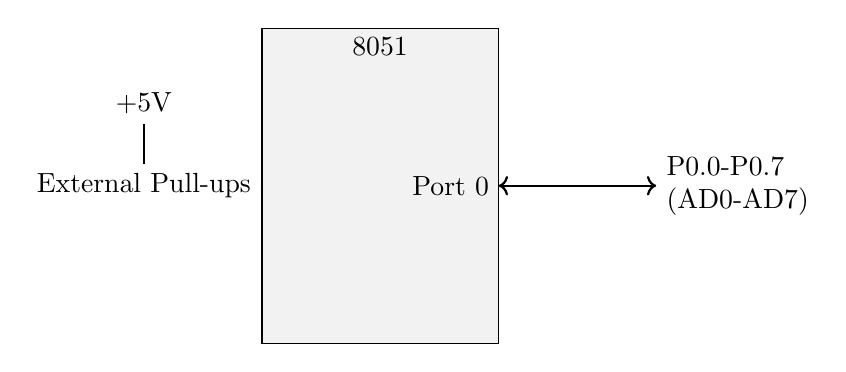
\begin{tikzpicture}[node distance=2cm, auto]
    % 8051 Chip
    \node [draw, rectangle, minimum width=3cm, minimum height=4cm, fill=black!5] (chip) {};
    \node [anchor=north] at (chip.north) {8051};
    \node [anchor=east] at (chip.east) {Port 0};
    
    % External Pull-ups
    \node [left of=chip, node distance=3cm] (pullup) {External Pull-ups};
    \draw [thick] (pullup.north) -- ++(0, 0.5) node[above] {+5V};
    \draw [thick] (pullup.east) -- (chip.west);
    
    % Port Lines
    \draw [<->, thick] (chip.east) -- ++(2,0) node[right, align=left] {P0.0-P0.7\\(AD0-AD7)};
\end{tikzpicture}
\end{center}
\end{solutionbox}
\begin{mnemonicbox}
``PORT 0-PLAD'' (Port 0 needs Pull-ups, works as Latch/Address/Data)
\end{mnemonicbox}

\questionmarks{1}{b}{4}
\textbf{Illustrate Microprocessor Architecture.}

\begin{solutionbox}
\textbf{Answer}:

\begin{center}
\captionof{table}{Microprocessor Components}
\begin{tabulary}{\linewidth}{|l|J|}
\hline
\textbf{Component} & \textbf{Function} \\ \hline
\textbf{ALU} & Performs arithmetic and logical operations \\ \hline
\textbf{Registers} & Temporary storage for data and addresses \\ \hline
\textbf{Control Unit} & Directs operation of processor and data flow \\ \hline
\textbf{Buses} & Pathways for data transfer (address, data, control) \\ \hline
\end{tabulary}
\end{center}

\textbf{Diagram:}

\begin{center}
\begin{tikzpicture}[node distance=2.5cm, auto]
    % CPU Box
    \node [draw, rectangle, minimum width=8cm, minimum height=6cm, rounded corners, fill=black!5] (cpu) {};
    \node [anchor=north west] at (cpu.north west) {\textbf{MICROPROCESSOR}};
    
    % Inside Components
    \node [gtu block, fill=white] (control) at ([xshift=2cm, yshift=1.5cm]cpu.center) {CONTROL UNIT\\Timing \& Control};
    \node [gtu block, fill=white] (regs) at ([xshift=-2cm, yshift=1.5cm]cpu.center) {REGISTERS\\A, B, C, D\\H, L, SP, PC};
    \node [gtu block, fill=white] (alu) at ([yshift=-1.5cm]cpu.center) {ALU};
    
    % Connections
    \draw [gtu arrow, <->] (regs) -- (control);
    \draw [gtu arrow, <->] (regs) -- (alu);
    \draw [gtu arrow, ->] (control) -- (alu);
    
    % Buses
    \node [gtu block, minimum width=6cm] (bus) [below of=alu, node distance=2cm] {ADDRESS, DATA \& CONTROL BUSES};
    \draw [gtu arrow, <->] (alu) -- (bus);
    
\end{tikzpicture}
\end{center}
\end{solutionbox}
\begin{mnemonicbox}
``RABC'' - ``Registers, ALU, Buses, Control''
\end{mnemonicbox}

\questionmarks{1}{c}{7}
\textbf{Compare Von Neumann \& Harvard architecture.}

\begin{solutionbox}
\textbf{Answer}:

\begin{center}
\captionof{table}{Von Neumann vs Harvard Architecture}
\begin{tabulary}{\linewidth}{|l|J|J|}
\hline
\textbf{Feature} & \textbf{Von Neumann Architecture} & \textbf{Harvard Architecture} \\ \hline
Memory Buses & Single memory bus for instructions and data & Separate buses for program and data memory \\ \hline
Execution & Sequential execution & Parallel fetch and execute possible \\ \hline
Speed & Slower due to bus bottleneck & Faster due to simultaneous access \\ \hline
Memory Access & Single memory space & Separate memory spaces \\ \hline
Complexity & Simpler design & More complex design \\ \hline
Applications & General-purpose computing & DSP, microcontrollers, embedded systems \\ \hline
Examples & Most PCs, 8085, 8086 & 8051, PIC, ARM Cortex-M \\ \hline
\end{tabulary}
\end{center}

\textbf{Diagram:}

\begin{center}
\begin{tikzpicture}[node distance=2cm]
    % Von Neumann
    \node (v_cpu) [gtu block] {CPU};
    \node (v_mem) [gtu block, right of=v_cpu, node distance=3.5cm] {Memory\\(Code + Data)};
    \draw [gtu arrow, <->] (v_cpu) -- node[above] {Bus} (v_mem);
    \node [below of=v_cpu, node distance=1.5cm] {\textbf{Von Neumann}};

    % Divider
    \draw [dashed] (5.5, 1) -- (5.5, -2);

    % Harvard
    \node (h_cpu) [gtu block, right of=v_mem, node distance=5cm] {CPU};
    \node (h_prog) [gtu block, right of=h_cpu, node distance=3.5cm, yshift=1cm] {Program\\Memory};
    \node (h_data) [gtu block, right of=h_cpu, node distance=3.5cm, yshift=-1cm] {Data\\Memory};
    \draw [gtu arrow, <->] (h_cpu) |- (h_prog);
    \draw [gtu arrow, <->] (h_cpu) |- (h_data);
    \node [below of=h_cpu, node distance=1.5cm] {\textbf{Harvard}};
\end{tikzpicture}
\end{center}
\end{solutionbox}
\begin{mnemonicbox}
``Harvard Has Separate Streets'' (Harvard Has Separate memory paths)
\end{mnemonicbox}

\orquestionmarks{1}{c}{7}
\textbf{Define RISC, CISC, Opcode, Operand, Instruction Cycle, Machine Cycle, and T State.}

\begin{solutionbox}
\textbf{Answer}:

\begin{center}
\captionof{table}{Definitions}
\begin{tabulary}{\linewidth}{|l|J|}
\hline
\textbf{Term} & \textbf{Definition} \\ \hline
\textbf{RISC} & Reduced Instruction Set Computer - architecture with simple instructions optimized for speed \\ \hline
\textbf{CISC} & Complex Instruction Set Computer - architecture with complex, powerful instructions \\ \hline
\textbf{Opcode} & Operation Code - part of instruction that specifies operation to be performed \\ \hline
\textbf{Operand} & Data value or address used in operation \\ \hline
\textbf{Instruction Cycle} & Complete process to fetch, decode and execute an instruction \\ \hline
\textbf{Machine Cycle} & Basic operation like memory read/write (subset of instruction cycle) \\ \hline
\textbf{T-State} & Time state - smallest unit of time in processor operation (clock period) \\ \hline
\end{tabulary}
\end{center}

\textbf{Diagram:}

\begin{center}
\begin{tikzpicture}[node distance=3cm, auto]
    % Instruction Cycle
    \node [gtu block] (fetch) {FETCH};
    \node [gtu block, right of=fetch] (decode) {DECODE};
    \node [gtu block, right of=decode] (execute) {EXECUTE};
    
    \draw [gtu arrow, ->] (fetch) -- (decode);
    \draw [gtu arrow, ->] (decode) -- (execute);
    \draw [gtu arrow, ->] (execute) -- ++(0,-1.5) -| (fetch);
    
    \node [below of=decode, node distance=2cm] {Instruction Cycle};
    
    % T-States
    \node [draw, rectangle, minimum width=1cm, minimum height=1cm] (t1) [below of=fetch, node distance=3.5cm] {T1};
    \node [draw, rectangle, minimum width=1cm, minimum height=1cm] (t2) [right of=t1, node distance=1cm] {T2};
    \node [draw, rectangle, minimum width=1cm, minimum height=1cm] (t3) [right of=t2, node distance=1cm] {T3};
    \node [draw, rectangle, minimum width=1cm, minimum height=1cm] (t4) [right of=t3, node distance=1cm] {T4};
    
    \draw [decorate, decoration={brace, amplitude=5pt}] (t1.south west) -- (t4.south east) node [midway, below=5pt] {Machine Cycle};
    
\end{tikzpicture}
\end{center}
\end{solutionbox}
\begin{mnemonicbox}
``RICO ITEM'' (RISC, CISC, Opcode, Instruction cycle, T-state, Execute, Machine cycle)
\end{mnemonicbox}

\questionmarks{2}{a}{3}
\textbf{Define Data bus, Address bus and Control bus.}

\begin{solutionbox}
\textbf{Answer}:

\begin{center}
\captionof{table}{Bus Definitions}
\begin{tabulary}{\linewidth}{|l|J|}
\hline
\textbf{Bus Type} & \textbf{Definition} \\ \hline
\textbf{Data Bus} & Bidirectional pathway that transfers actual data between microprocessor and peripheral devices \\ \hline
\textbf{Address Bus} & Unidirectional pathway that carries memory/IO device locations to be accessed \\ \hline
\textbf{Control Bus} & Group of signal lines that coordinate and synchronize all system operations \\ \hline
\end{tabulary}
\end{center}

\textbf{Diagram:}

\begin{center}
\begin{tikzpicture}[node distance=2.5cm, auto]
    \node [gtu block] (cpu) {CPU};
    
    \draw [->, thick] (cpu.east) -- ++(2,1) node[right] {Address Bus (Unidirectional)};
    \draw [<->, thick] (cpu.east) -- ++(2,0) node[right] {Data Bus (Bidirectional)};
    \draw [->, thick] (cpu.east) -- ++(2,-1) node[right] {Control Bus (Signals)};
\end{tikzpicture}
\end{center}
\end{solutionbox}
\begin{mnemonicbox}
``ADC'' - ``Address finds location, Data carries information, Control coordinates operations''
\end{mnemonicbox}

\questionmarks{2}{b}{4}
\textbf{Compare Microprocessor and Microcontroller.}

\begin{solutionbox}
\textbf{Answer}:

\begin{center}
\captionof{table}{Microprocessor vs Microcontroller}
\begin{tabulary}{\linewidth}{|l|J|J|}
\hline
\textbf{Feature} & \textbf{Microprocessor} & \textbf{Microcontroller} \\ \hline
Definition & CPU on a single chip & Complete computer system on a chip \\ \hline
Memory & External RAM/ROM needed & Built-in RAM/ROM \\ \hline
I/O Ports & Limited or none on-chip & Multiple I/O ports on-chip \\ \hline
Peripherals & External peripherals needed & Built-in peripherals (timers, ADC, etc.) \\ \hline
Applications & General computing, PCs & Embedded systems, IoT devices \\ \hline
Cost & Higher for complete system & Lower (all-in-one solution) \\ \hline
Power & Higher & Lower \\ \hline
\end{tabulary}
\end{center}
\end{solutionbox}
\begin{mnemonicbox}
``MEMI-CAP'' (Memory external/internal, Cost, Applications, Peripherals)
\end{mnemonicbox}

\questionmarks{2}{c}{7}
\textbf{Sketch and explain 8085 block diagram.}

\begin{solutionbox}
\textbf{Answer}:

\textbf{Diagram:}

\begin{center}
\begin{tikzpicture}[node distance=2cm, scale=0.8, transform shape]
    % Outer Box
    \node [draw, rectangle, minimum width=10cm, minimum height=8cm, rounded corners, fill=black!5] (cpu) {};
    \node [anchor=north] at (cpu.north) {\textbf{8085 CPU}};
    
    % Internal Registers
    \node [gtu block, fill=white] (regs) at ([xshift=-3cm, yshift=2cm]cpu.center) {REGISTER ARRAY\\B,C, D,E, H,L\\SP, PC};
    
    % ALU
    \node [gtu block, fill=white] (alu) at ([xshift=-3cm, yshift=-1cm]cpu.center) {ALU};
    
    % Accumulator & Flags
    \node [gtu block, fill=white] (acc) at ([yshift=1.5cm]alu.north) {A | Flags};
    
    % Timing & Control
    \node [gtu block, fill=white] (control) at ([xshift=3cm, yshift=2cm]cpu.center) {TIMING \&\\CONTROL};
    \node [gtu block, fill=white] (decoder) at ([yshift=-1.5cm]control.south) {Instruction\\Decoder};
    
    % Buses
    \node [gtu block, minimum width=8cm] (intbus) at ([yshift=-2.5cm]alu.south) {INTERNAL DATA BUS};
    
    % Connections
    \draw [gtu arrow, <->] (regs) -- (intbus);
    \draw [gtu arrow, <->] (alu) -- (intbus);
    \draw [gtu arrow, <->] (acc) -- (alu);
    \draw [gtu arrow, <->] (control) -- (decoder);
    \draw [gtu arrow] (decoder) -| (alu);
    
    % External Interface
    \node [gtu block, fill=white, below of=intbus] (interface) {Address/Data Buffers};
    \draw [gtu arrow, <->] (intbus) -- (interface);
    
    \draw [->, thick] (interface.south) -- ++(0,-1) node[below] {Address/Data Bus};
    \draw [->, thick] (control.east) -- ++(1,0) node[right] {Control Signals};

\end{tikzpicture}
\end{center}

\textbf{Main Components:}
\begin{itemize}
\item \textbf{Register Array}: A (Accumulator), Flags, B-L, SP, PC, temp registers
\item \textbf{ALU}: Performs arithmetic and logical operations
\item \textbf{Timing \& Control}: Generates control signals, handles interrupts
\item \textbf{Bus Interface}: Connects CPU to external devices
\item \textbf{Internal Data Bus}: Links internal components
\end{itemize}
\end{solutionbox}
\begin{mnemonicbox}
``RATBI'' - ``Registers, ALU, Timing, Buses, Interface''
\end{mnemonicbox}

\orquestionmarks{2}{a}{3}
\textbf{Explain Accumulator, Program Counter and Stack Pointer.}

\begin{solutionbox}
\textbf{Answer}:

\begin{center}
\captionof{table}{Register Functions}
\begin{tabulary}{\linewidth}{|l|J|}
\hline
\textbf{Register} & \textbf{Function} \\ \hline
\textbf{Accumulator (A)} & 8-bit register that stores results of arithmetic and logical operations \\ \hline
\textbf{Program Counter (PC)} & 16-bit register that holds address of next instruction to be executed \\ \hline
\textbf{Stack Pointer (SP)} & 16-bit register that points to current top of stack in memory \\ \hline
\end{tabulary}
\end{center}

\textbf{Diagram:}

\begin{center}
\begin{tikzpicture}[node distance=2cm, auto]
    % Accumulator
    \node [gtu block] (acc) {Accumulator (A)\\Data Ops};
    
    % PC
    \node [gtu block, right of=acc, node distance=4cm] (pc) {Program Counter\\(PC)};
    \node [right of=pc, node distance=2.5cm, align=left] {$\to$ Next\\Instruction};
    
    % SP
    \node [gtu block, right of=pc, node distance=5cm] (sp) {Stack Pointer\\(SP)};
    \node [gtu block, below of=sp, node distance=2cm] (stack) {Stack Memory};
    
    \draw [->, thick] (sp) -- (stack) node[midway, right] {Points Top};
\end{tikzpicture}
\end{center}
\end{solutionbox}
\begin{mnemonicbox}
``APS'' - ``Accumulator Processes, PC Predicts, SP Stacks''
\end{mnemonicbox}

\orquestionmarks{2}{b}{4}
\textbf{Sketch and explain Demultiplexing of Address bus and data bus.}

\begin{solutionbox}
\textbf{Answer}:

\textbf{Diagram:}

\begin{center}
\begin{tikzpicture}[node distance=2.5cm, auto]
    \node [gtu block, minimum width=3cm, minimum height=4cm] (cpu) {8085 CPU};
    \node [gtu block, right of=cpu, node distance=5cm, yshift=-1.5cm] (latch) {74LS373\\Latch};
    
    % Higher Address
    \draw [->, thick] (cpu.east) ++(0, 0.5) -- ++(3,0) node[right] {A15-A8 (Higher Address)};
    
    % AD7-AD0 (Multiplexed)
    \draw [thick] (cpu.east) ++(0, -1.5) -- (latch.west) node[midway, above] {AD7-AD0};
    
    % Data Bus Drop
    \draw [<->, thick] ($(cpu.east)!0.5!(latch.west)$) -- ++(0, -2) node[below] {Data Bus D7-D0};
    
    % ALE
    \draw [->, thick] (cpu.east) ++(0, -2.5) -- (latch.south west) node[midway, right] {ALE};
    
    % Lower Address Output
    \draw [->, thick] (latch.east) -- ++(2,0) node[right] {A7-A0 (Lower Address)};
    
\end{tikzpicture}
\end{center}

\textbf{Process}:
\begin{enumerate}
\item \textbf{Multiplexing}: AD0-AD7 pins share address and data signals to reduce pin count.
\item \textbf{Demultiplexing Steps}:
    \begin{itemize}
    \item CPU places address on AD0-AD7 pins.
    \item ALE (Address Latch Enable) signal goes HIGH.
    \item External latch (74LS373) captures lower address bits.
    \item ALE goes LOW, latching the address.
    \item AD0-AD7 pins now carry data.
    \end{itemize}
\end{enumerate}
\end{solutionbox}
\begin{mnemonicbox}
``ALAD'' - ``ALE Active, Latch Address, After Data''
\end{mnemonicbox}

\orquestionmarks{2}{c}{7}
\textbf{List any seven features of 8085.}

\begin{solutionbox}
\textbf{Answer}:

\begin{center}
\captionof{table}{8085 Features}
\begin{tabulary}{\linewidth}{|l|J|}
\hline
\textbf{Feature} & \textbf{Description} \\ \hline
\textbf{8-bit Data Bus} & Transfers 8 bits of data in parallel \\ \hline
\textbf{16-bit Address Bus} & Can address up to 64KB of memory ($2^{16}$) \\ \hline
\textbf{Hardware Interrupts} & 5 hardware interrupts (TRAP, RST 7.5, 6.5, 5.5, INTR) \\ \hline
\textbf{Serial I/O} & SID and SOD pins for serial communication \\ \hline
\textbf{Clock Generation} & On-chip clock generator with crystal \\ \hline
\textbf{Instruction Set} & 74 operation codes generating 246 instructions \\ \hline
\textbf{Register Set} & Six 8-bit registers (B,C,D,E,H,L), accumulator, flags, SP, PC \\ \hline
\end{tabulary}
\end{center}

\textbf{Diagram:}

\begin{center}
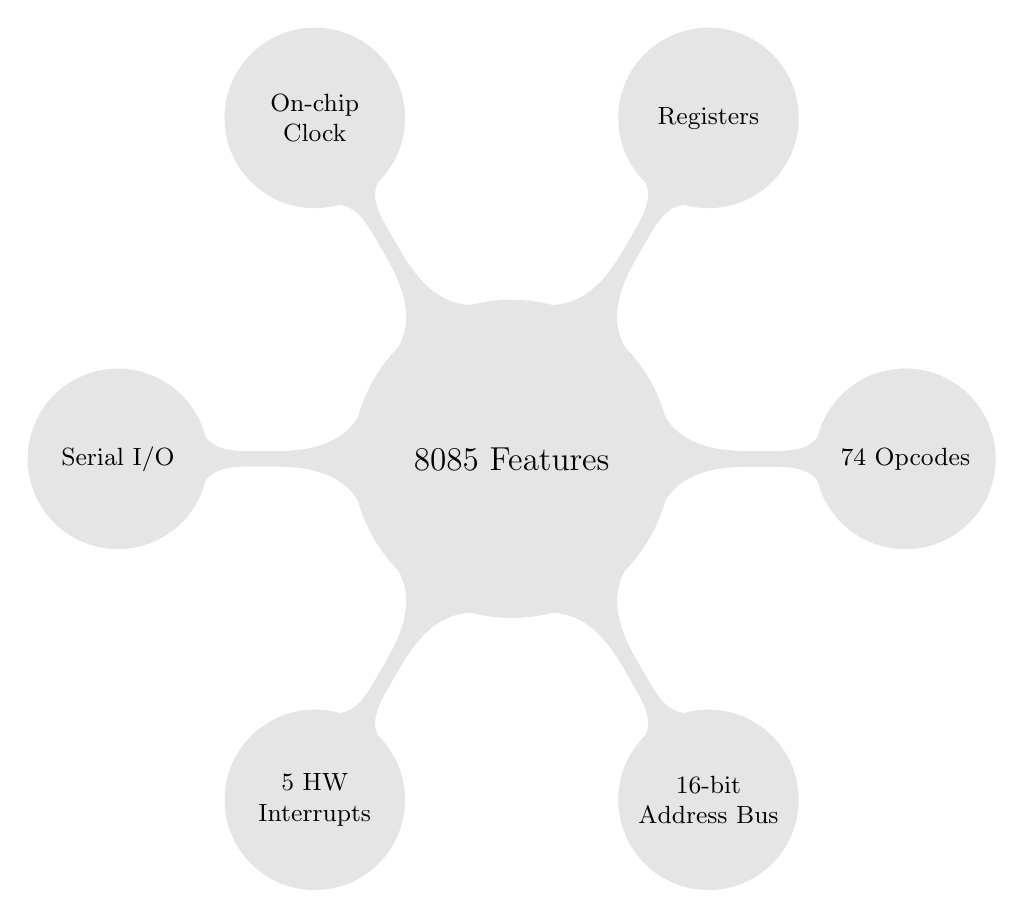
\begin{tikzpicture}
  \path[mindmap,concept color=black!10,text=black]
    node[concept] {8085 Features}
    [clockwise from=0]
    child { node[concept] {8-bit Data Bus} }
    child { node[concept] {16-bit Address Bus} }
    child { node[concept] {5 HW Interrupts} }
    child { node[concept] {Serial I/O} }
    child { node[concept] {On-chip Clock} }
    child { node[concept] {Registers} }
    child { node[concept] {74 Opcodes} };
\end{tikzpicture}
\end{center}
\end{solutionbox}
\begin{mnemonicbox}
``CHAIRS'' - ``Clock, Hardware interrupts, Address bus, Instruction set, Registers, Serial I/O''
\end{mnemonicbox}

\questionmarks{3}{a}{3}
\textbf{Illustrate any one Timer Mode of 8051.}

\begin{solutionbox}
\textbf{Answer}:

\textbf{Mode 1: 16-bit Timer/Counter}

\begin{center}
\captionof{table}{Timer Mode 1}
\begin{tabulary}{\linewidth}{|l|J|}
\hline
\textbf{Feature} & \textbf{Description} \\ \hline
\textbf{Timer Structure} & 16-bit timer using THx and TLx registers \\ \hline
\textbf{Operation} & Counts from 0000H to FFFFH, then sets TF flag \\ \hline
\textbf{Counter Size} & Full 16-bit counter ($2^{16} = 65,536$ counts) \\ \hline
\textbf{Registers} & THx (high byte) and TLx (low byte) \\ \hline
\end{tabulary}
\end{center}

\textbf{Diagram:}

\begin{center}
\begin{tikzpicture}[auto, node distance=2.5cm]
    \node [gtu block] (control) {Control Bits};
    \node [gtu block, right of=control, node distance=3cm] (gate) {Gate Control};
    \node [gtu block, right of=gate, node distance=3cm] (overflow) {Overflow\\Detect};
    
    \node [right of=overflow, node distance=2.5cm] (flag) {TF (Flag)};
    \draw [->, thick] (overflow) -- (flag);
    
    \draw [->, thick] (control) -- (gate);
    \draw [->, thick] (gate) -- (overflow);
    
    \node [gtu block, below of=gate, node distance=2cm] (counter) {THx:TLx Counter\\(16-bit)};
    \node [left of=counter, node distance=3cm] (clock) {Clock Source};
    
    \draw [->, thick] (clock) -- (counter);
    \draw [->, thick] (counter) -| (overflow);
    \draw [dashed] (gate) -- (counter);

\end{tikzpicture}
\end{center}
\end{solutionbox}
\begin{mnemonicbox}
``MOGC'' - ``Mode 1 uses Overflow detection, Gate control, Complete 16-bits''
\end{mnemonicbox}

\questionmarks{3}{b}{4}
\textbf{State function of ALE, PSEN, RESET and TXD pin for 8051.}

\begin{solutionbox}
\textbf{Answer}:

\begin{center}
\captionof{table}{Pin Functions}
\begin{tabulary}{\linewidth}{|l|J|}
\hline
\textbf{Pin} & \textbf{Function} \\ \hline
\textbf{ALE} & Address Latch Enable - Provides control signal to latch low byte of address from port 0 \\ \hline
\textbf{PSEN} & Program Store Enable - Read strobe for external program memory access \\ \hline
\textbf{RESET} & Reset input - Forces CPU to initial state when held HIGH for 2 machine cycles \\ \hline
\textbf{TXD} & Transmit Data - Serial port output pin for serial data transmission \\ \hline
\end{tabulary}
\end{center}

\textbf{Diagram:}

\begin{center}
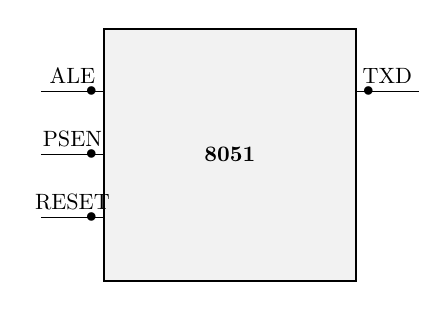
\begin{tikzpicture}[scale=0.8, transform shape]
    \draw[thick, fill=black!5] (0,0) rectangle (4,4);
    \node at (2,2) {\textbf{8051}};
    
    \draw (-1, 3) -- (0, 3) node[midway, above] {ALE};
    \draw (-1, 2) -- (0, 2) node[midway, above] {PSEN};
    \draw (-1, 1) -- (0, 1) node[midway, above] {RESET};
    \draw (4, 3) -- (5, 3) node[midway, above] {TXD};
    
    \node at (-0.2, 3) {$\bullet$};
    \node at (-0.2, 2) {$\bullet$};
    \node at (-0.2, 1) {$\bullet$};
    \node at (4.2, 3) {$\bullet$};
\end{tikzpicture}
\end{center}
\end{solutionbox}
\begin{mnemonicbox}
``APTR'' - ``Address latch, Program store, Total reset, tRansmit data''
\end{mnemonicbox}

\questionmarks{3}{c}{7}
\textbf{Explain functions of each block of 8051 Microcontroller.}

\begin{solutionbox}
\textbf{Answer}:

\begin{center}
\captionof{table}{8051 Blocks}
\begin{tabulary}{\linewidth}{|l|J|}
\hline
\textbf{Block} & \textbf{Function} \\ \hline
\textbf{CPU} & 8-bit processor that fetches and executes instructions \\ \hline
\textbf{Memory} & 4KB internal ROM and 128 bytes of internal RAM \\ \hline
\textbf{I/O Ports} & Four 8-bit bidirectional I/O ports (P0-P3) \\ \hline
\textbf{Timers/Counters} & Two 16-bit timers/counters for timing and counting \\ \hline
\textbf{Serial Port} & Full-duplex UART for serial communication \\ \hline
\textbf{Interrupts} & Five interrupt sources with two priority levels \\ \hline
\textbf{Clock Circuit} & Provides timing for all operations \\ \hline
\end{tabulary}
\end{center}

\textbf{Diagram:}

\begin{center}
\begin{tikzpicture}[node distance=2.5cm, auto]
    % CPU
    \node [gtu block, fill=white] (cpu) {CPU};
    
    % Peripherals
    \node [gtu block, right of=cpu, node distance=4cm] (timers) {Timers/\\Counters};
    \node [gtu block, right of=timers, node distance=3.5cm] (interrupts) {Interrupts};
    
    \node [gtu block, below of=cpu, node distance=3cm] (memory) {Memory\\RAM/ROM};
    \node [gtu block, right of=memory, node distance=4cm] (serial) {Serial\\Port};
    \node [gtu block, right of=serial, node distance=3.5cm] (ports) {I/O Ports\\P0-P3};
    
    % Clock
    \node [gtu block, minimum width=8cm, below of=memory, node distance=2.5cm, xshift=2cm] (clock) {Clock Circuit};
    
    % Connections
    \draw [gtu arrow, <->] (cpu) -- (timers);
    \draw [gtu arrow, <->] (cpu) -| (interrupts);
    \draw [gtu arrow, <->] (cpu) -- (memory);
    \draw [gtu arrow, <->] (memory) -- (serial);
    \draw [gtu arrow, <->] (serial) -- (ports);
    \draw [gtu arrow, ->] (clock) -- ++(0,1.5);
    
    \node [draw, dashed, fit=(cpu) (ports) (clock)] {};
    \node [above] at (cpu.north) {\textbf{8051 ARCHITECTURE}};

\end{tikzpicture}
\end{center}
\end{solutionbox}
\begin{mnemonicbox}
``CRIMSON'' - ``CPU, RAM/ROM, I/O, Memory, Serial port, Oscillator, iNterrupts''
\end{mnemonicbox}

\orquestionmarks{3}{a}{3}
\textbf{Illustrate any one Serial Communication Mode of 8051.}

\begin{solutionbox}
\textbf{Answer}:

\textbf{Mode 1: 8-bit UART}

\begin{center}
\captionof{table}{Serial Mode 1}
\begin{tabulary}{\linewidth}{|l|J|}
\hline
\textbf{Feature} & \textbf{Description} \\ \hline
\textbf{Format} & 10 bits (start bit, 8 data bits, stop bit) \\ \hline
\textbf{Baud Rate} & Variable, determined by Timer 1 \\ \hline
\textbf{Data Direction} & Full-duplex (simultaneous transmit and receive) \\ \hline
\textbf{Pins Used} & TXD (P3.1) for transmit, RXD (P3.0) for receive \\ \hline
\end{tabulary}
\end{center}

\textbf{Diagram:}

\begin{center}
\begin{tikzpicture}[node distance=2.5cm, auto]
    \node [gtu block] (timer) {Timer 1};
    \node [gtu block, right of=timer, node distance=3.5cm] (baud) {Baud Rate\\Generator};
    \node [gtu block, right of=baud, node distance=3.5cm] (tx) {Transmit\\Shift Reg};
    
    \draw [->, thick] (timer) -- (baud);
    \draw [->, thick] (baud) -- (tx);
    \draw [->, thick] (tx) -- ++(2,0) node[right] {Serial Out (TXD)};
    
    \node [gtu block, below of=tx, node distance=2.5cm] (rx) {Receive\\Shift Reg};
    \draw [<-, thick] (rx) -- ++(2,0) node[right] {Serial In (RXD)};
    
    \node [gtu block, above of=tx, node distance=2cm] (sbuf) {SBUF};
    \draw [->, thick] (sbuf) -- (tx);
    \draw [->, thick] (rx) -- ++(-2,0) |- (sbuf);

\end{tikzpicture}
\end{center}
\end{solutionbox}
\begin{mnemonicbox}
``FADS'' - ``Format 10-bit, Auto baud from Timer 1, Duplex mode, Standard UART''
\end{mnemonicbox}

\orquestionmarks{3}{b}{4}
\textbf{State function of RXD, INT0, T0 and PROG pin for 8051.}

\begin{solutionbox}
\textbf{Answer}:

\begin{center}
\captionof{table}{Pin Functions}
\begin{tabulary}{\linewidth}{|l|J|}
\hline
\textbf{Pin} & \textbf{Function} \\ \hline
\textbf{RXD (P3.0)} & Receive Data - Serial port input pin for serial data reception \\ \hline
\textbf{INT0 (P3.2)} & External Interrupt 0 - Input that can trigger external interrupt \\ \hline
\textbf{T0 (P3.4)} & Timer 0 - External count input for Timer/Counter 0 \\ \hline
\textbf{PROG (EA)} & Program Enable - When LOW, forces CPU to fetch code from external memory \\ \hline
\end{tabulary}
\end{center}

\textbf{Diagram:}

\begin{center}
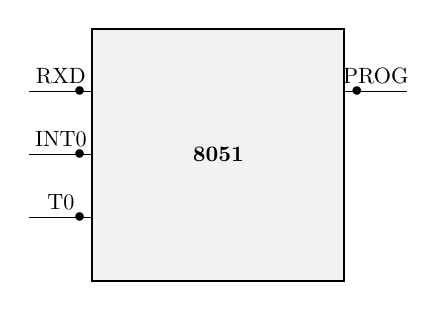
\begin{tikzpicture}[scale=0.8, transform shape]
    \draw[thick, fill=black!5] (0,0) rectangle (4,4);
    \node at (2,2) {\textbf{8051}};
    
    \draw (-1, 3) -- (0, 3) node[midway, above] {RXD};
    \draw (-1, 2) -- (0, 2) node[midway, above] {INT0};
    \draw (-1, 1) -- (0, 1) node[midway, above] {T0};
    \draw (4, 3) -- (5, 3) node[midway, above] {PROG};
    
    \node at (-0.2, 3) {$\bullet$};
    \node at (-0.2, 2) {$\bullet$};
    \node at (-0.2, 1) {$\bullet$};
    \node at (4.2, 3) {$\bullet$};
\end{tikzpicture}
\end{center}
\end{solutionbox}
\begin{mnemonicbox}
``RIPE'' - ``Receive data, Interrupt trigger, Pulse counting, External memory''
\end{mnemonicbox}

\orquestionmarks{3}{c}{7}
\textbf{Describe ALU, PC, DPTR, RS0, RS1, Internal RAM and Internal ROM of 8051.}

\begin{solutionbox}
\textbf{Answer}:

\begin{center}
\captionof{table}{Register/Memory Description}
\begin{tabulary}{\linewidth}{|l|J|}
\hline
\textbf{Component} & \textbf{Description} \\ \hline
\textbf{ALU} & Arithmetic Logic Unit - Performs math and logical operations \\ \hline
\textbf{PC} & Program Counter - 16-bit register that points to next instruction \\ \hline
\textbf{DPTR} & Data Pointer - 16-bit register (DPH+DPL) for external memory addressing \\ \hline
\textbf{RS0, RS1} & Register Bank Select bits in PSW - Select one of four register banks \\ \hline
\textbf{Internal RAM} & 128 bytes on-chip RAM (00H-7FH) for variables and stack \\ \hline
\textbf{Internal ROM} & 4KB on-chip ROM (0000H-0FFFH) for program storage \\ \hline
\end{tabulary}
\end{center}

\textbf{Diagram:}

\begin{center}
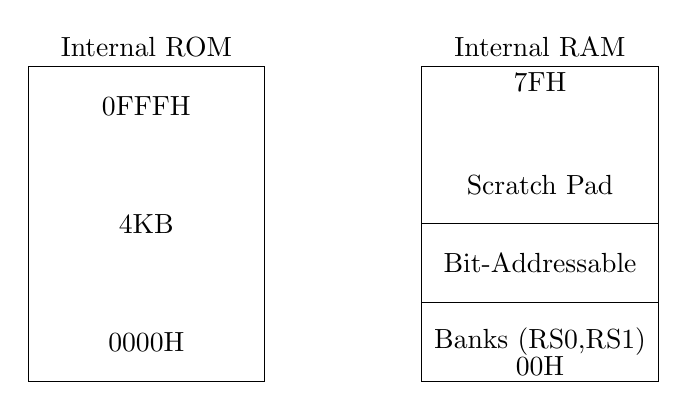
\begin{tikzpicture}[node distance=2cm]
    % ROM
    \node [draw, rectangle, minimum width=3cm, minimum height=4cm, label=above:Internal ROM] (rom) at (0,0) {};
    \node at (0, 1.5) {0FFFH};
    \node at (0, -1.5) {0000H};
    \node at (0, 0) {4KB};
    
    % RAM
    \node [draw, rectangle, minimum width=3cm, minimum height=4cm, label=above:Internal RAM] (ram) at (5,0) {};
    \node at (5, 1.8) {7FH};
    \node at (5, 0.5) {Scratch Pad};
    \draw (3.5, 0) -- (6.5, 0);
    \node at (5, -0.5) {Bit-Addressable};
    \draw (3.5, -1) -- (6.5, -1);
    \node at (5, -1.5) {Banks (RS0,RS1)};
    \node at (5, -1.8) {00H};
    
\end{tikzpicture}
\end{center}
\end{solutionbox}
\begin{mnemonicbox}
``APRID'' - ``ALU Processes, PC Remembers, Register bank select, Internal memory, DPTR points''
\end{mnemonicbox}

\questionmarks{4}{a}{3}
\textbf{Develop an Assembly language program to divide 08H by 02H.}

\begin{solutionbox}
\textbf{Answer}:

\begin{lstlisting}[language={[x86masm]Assembler}]
      MOV A, #08H    ; Load dividend 08H into accumulator
      MOV B, #02H    ; Load divisor 02H into B register
      DIV AB         ; Divide A by B (A=quotient, B=remainder)
      MOV R0, A      ; Store quotient in R0 (04H)
      MOV R1, B      ; Store remainder in R1 (00H)
\end{lstlisting}

\textbf{Diagram:}

\begin{center}
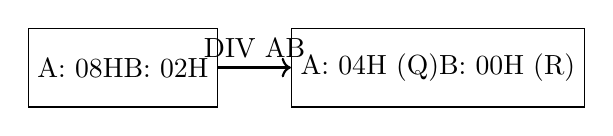
\begin{tikzpicture}[node distance=2cm]
    \node [draw, rectangle, minimum width=2cm, minimum height=1cm] (before) {A: 08H\\B: 02H};
    \node [draw, rectangle, minimum width=2cm, minimum height=1cm, right of=before, node distance=4cm] (after) {A: 04H (Q)\\B: 00H (R)};
    \draw [->, thick] (before) -- (after) node[midway, above] {DIV AB};
\end{tikzpicture}
\end{center}
\end{solutionbox}
\begin{mnemonicbox}
``LDDS'' - ``Load dividend, Divisor in B, Divide, Store results''
\end{mnemonicbox}

\questionmarks{4}{b}{4}
\textbf{Develop an Assembly language program to add 76H and 32H.}

\begin{solutionbox}
\textbf{Answer}:

\begin{lstlisting}[language={[x86masm]Assembler}]
      MOV A, #76H    ; Load first number 76H into accumulator
      MOV R0, #32H   ; Load second number 32H into R0
      ADD A, R0      ; Add R0 to A (76H + 32H = A8H)
      MOV R1, A      ; Store result in R1 (A8H)
      JNC DONE       ; Jump if no carry
      MOV R2, #01H   ; If carry occurred, store 1 in R2
DONE: NOP            ; End program
\end{lstlisting}

\textbf{Calculation:}
\begin{center}
\begin{tabular}{r c l}
  76H & = & 0111 0110 \\
+ 32H & = & 0011 0010 \\
\hline
  A8H & = & 1010 1000 \\
\end{tabular}
\end{center}
\end{solutionbox}
\begin{mnemonicbox}
``LASER'' - ``Load A, Store second number, Execute addition, Result stored''
\end{mnemonicbox}

\questionmarks{4}{c}{7}
\textbf{What is Addressing mode? Classify it for 8051.}

\begin{solutionbox}
\textbf{Answer}:

\textbf{Addressing Mode}: Method to specify the location of operand/data for an instruction.

\begin{center}
\captionof{table}{Addressing Modes}
\begin{tabulary}{\linewidth}{|l|l|J|}
\hline
\textbf{Mode} & \textbf{Example} & \textbf{Description} \\ \hline
\textbf{Register} & \code{MOV A, R0} & Operand in register \\ \hline
\textbf{Direct} & \code{MOV A, 30H} & Operand at specific memory location (30H) \\ \hline
\textbf{Register Indirect} & \code{MOV A, @R0} & Register (R0) contains address of operand \\ \hline
\textbf{Immediate} & \code{MOV A, \#55H} & Operand (\#55H) is part of instruction \\ \hline
\textbf{Indexed} & \code{MOVC A, @A+DPTR} & Base address (DPTR) + offset (A) \\ \hline
\textbf{Bit} & \code{SETB P1.0} & Individual bit addressable \\ \hline
\textbf{Implied} & \code{RRC A} & Operand implied by instruction \\ \hline
\end{tabulary}
\end{center}

\textbf{Diagram:}

\begin{center}
\begin{tikzpicture}[node distance=3cm]
    \node [gtu block] (immed) {Immediate\\\#Data};
    \node [gtu block, right of=immed] (direct) {Direct\\Address};
    \node [gtu block, right of=direct] (reg) {Register\\Rn};
    
    \node [gtu block, below of=immed, node distance=2cm] (indirect) {Indirect\\@Rn};
    \node [gtu block, right of=indirect] (index) {Indexed\\@A+DPTR};
    
    \node [draw, fit=(immed) (index), label=above:Address Modes] {};
\end{tikzpicture}
\end{center}
\end{solutionbox}
\begin{mnemonicbox}
``RIDDIB'' - ``Register, Immediate, Direct, Data indirect, Indexed, Bit''
\end{mnemonicbox}

\orquestionmarks{4}{a}{3}
\textbf{Develop an Assembly language program to multiply 08H and 02H.}

\begin{solutionbox}
\textbf{Answer}:

\begin{lstlisting}[language={[x86masm]Assembler}]
      MOV A, #08H    ; Load first number 08H into accumulator
      MOV B, #02H    ; Load second number 02H into B register
      MUL AB         ; Multiply A and B (B:A = result)
      MOV R0, A      ; Store low-byte result in R0 (10H)
      MOV R1, B      ; Store high-byte result in R1 (00H)
\end{lstlisting}

\textbf{Diagram:}

\begin{center}
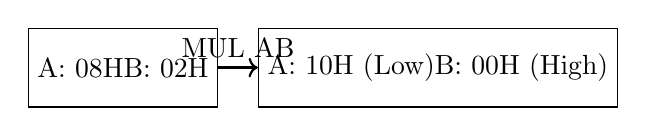
\begin{tikzpicture}[node distance=2cm]
    \node [draw, rectangle, minimum width=2cm, minimum height=1cm] (before) {A: 08H\\B: 02H};
    \node [draw, rectangle, minimum width=2cm, minimum height=1cm, right of=before, node distance=4cm] (after) {A: 10H (Low)\\B: 00H (High)};
    \draw [->, thick] (before) -- (after) node[midway, above] {MUL AB};
\end{tikzpicture}
\end{center}
\end{solutionbox}
\begin{mnemonicbox}
``LMSR'' - ``Load numbers, Multiply, Store Result''
\end{mnemonicbox}

\orquestionmarks{4}{b}{4}
\textbf{Develop an Assembly language program to subtract 76H from 32H.}

\begin{solutionbox}
\textbf{Answer}:

\begin{lstlisting}[language={[x86masm]Assembler}]
      MOV A, #32H    ; Load 32H into accumulator
      MOV R0, #76H   ; Load 76H into R0
      CLR C          ; Clear carry flag (borrow flag)
      SUBB A, R0     ; Subtract R0 from A with borrow (32H - 76H = BCH)
      MOV R1, A      ; Store result in R1 (BCH, which represents -44H)
\end{lstlisting}

\textbf{Calculation:}
\begin{center}
\begin{tabular}{r c l}
  32H & = & 0011 0010 \\
- 76H & = & 0111 0110 \\
\hline
  BCH & = & 1011 1100 (Two's complement) \\
\end{tabular}
\end{center}
\end{solutionbox}
\begin{mnemonicbox}
``LESS'' - ``Load first number, Enable borrow (CLR C), Subtract, Store''
\end{mnemonicbox}

\orquestionmarks{4}{c}{7}
\textbf{List types of instruction set. Explain any three with one example.}

\begin{solutionbox}
\textbf{Answer}:

\begin{center}
\captionof{table}{Instruction Types}
\begin{tabulary}{\linewidth}{|l|J|l|}
\hline
\textbf{Group} & \textbf{Description} & \textbf{Example} \\ \hline
\textbf{Arithmetic} & Mathematical operations & \code{ADD A, R0} \\ \hline
\textbf{Logical} & Logical operations & \code{ANL A, \#0FH} \\ \hline
\textbf{Data Transfer} & Move data between locations & \code{MOV A, R7} \\ \hline
\textbf{Branch} & Change program flow & \code{JNZ LOOP} \\ \hline
\textbf{Bit Manipulation} & Operate on individual bits & \code{SETB P1.0} \\ \hline
\textbf{Machine Control} & Control processor operation & \code{NOP} \\ \hline
\end{tabulary}
\end{center}

\textbf{Explanation}:
\begin{enumerate}
    \item \textbf{Data Transfer Instructions}:
    \begin{itemize}
        \item Move data between registers, memory, or I/O ports.
        \item Example: \code{MOV A, 30H} (Move data from memory 30H to A).
    \end{itemize}
    \item \textbf{Arithmetic Instructions}:
    \begin{itemize}
        \item Perform mathematical operations.
        \item Example: \code{ADD A, R0} (Add content of R0 to A).
    \end{itemize}
    \item \textbf{Logical Instructions}:
    \begin{itemize}
        \item Perform logical operations (AND, OR, XOR).
        \item Example: \code{ANL A, \#0FH} (AND A with 0FH).
    \end{itemize}
\end{enumerate}

\textbf{Diagram:}

\begin{center}
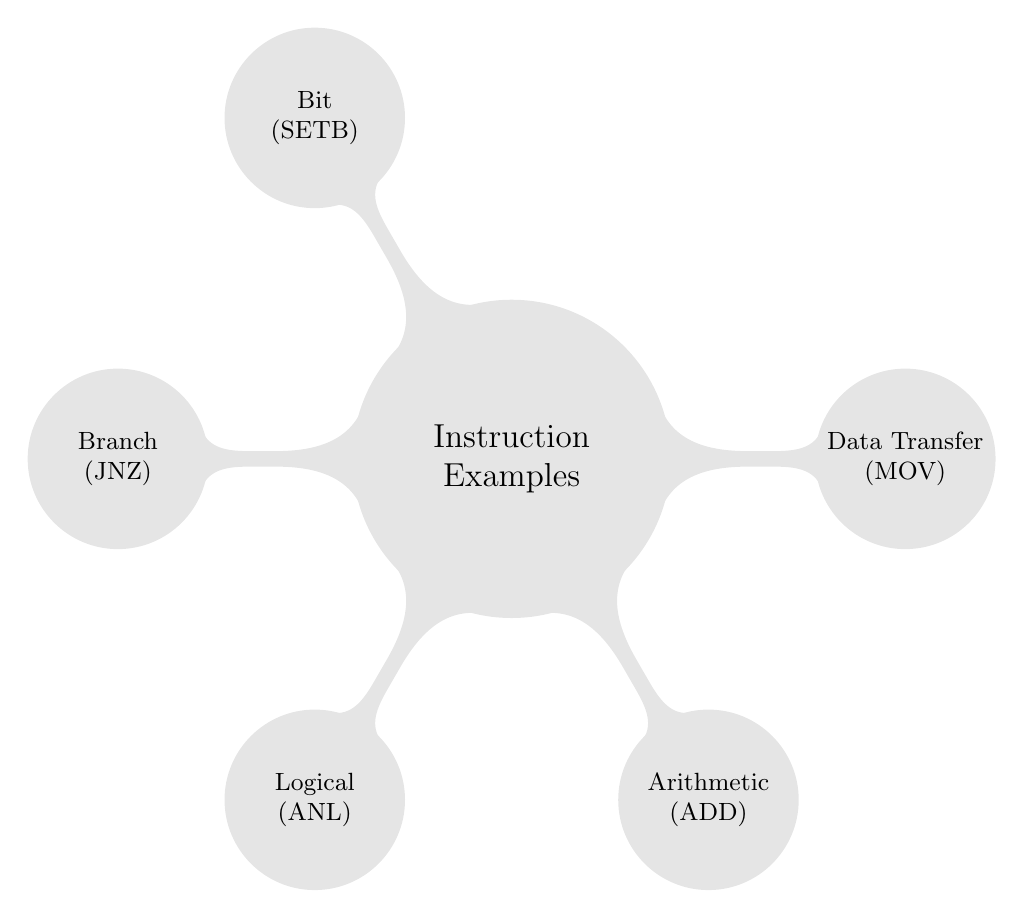
\begin{tikzpicture}
  \path[mindmap,concept color=black!10,text=black]
    node[concept] {Instruction Examples}
    [clockwise from=0]
    child { node[concept] {Data Transfer\\(MOV)} }
    child { node[concept] {Arithmetic\\(ADD)} }
    child { node[concept] {Logical\\(ANL)} }
    child { node[concept] {Branch\\(JNZ)} }
    child { node[concept] {Bit\\(SETB)} };
\end{tikzpicture}
\end{center}
\end{solutionbox}
\begin{mnemonicbox}
``BALDM'' - ``Branch, Arithmetic, Logical, Data transfer, Machine control''
\end{mnemonicbox}

\questionmarks{5}{a}{3}
\textbf{Sketch interfacing of four LEDs with 8051 Microcontroller.}

\begin{solutionbox}
\textbf{Answer}:

\textbf{Diagram:}

\begin{center}
\begin{tikzpicture}[node distance=2.5cm]
    \node [gtu block, minimum width=6cm] (8051) {8051 Microcontroller};
    
    \foreach \i in {0,1,2,3} {
        \node (p\i) at (-1.5 + \i, 1) {\scriptsize P1.\i};
        \draw [<-] (p\i.north) -- ++(0, 0.5) coordinate (mid\i);
        \draw (mid\i) -- ++(0, 0.5) node[midway, draw, rectangle, minimum width=0.3cm, minimum height=0.6cm, fill=white] {} coordinate (led\i); % LED symbol placeholder
        \node at (led\i) {\tiny LED};
        \draw (led\i) ++(0, 0.3) -- ++(0, 0.5) node[midway, draw, rectangle, minimum width=0.2cm, minimum height=0.5cm] {}; % Resistor
        \node at ($(led\i)+(0.5,0.6)$) {\tiny $220\Omega$};
        \draw ($(led\i)+(0, 0.8)$) -- ++(0, 0.2) node[above] {+5V};
    }
\end{tikzpicture}
\end{center}

\textbf{Details}:
\begin{itemize}
    \item LEDs connected to Port 1 (P1.0-P1.3).
    \item Common Anode configuration (Active Low) shown (Current flows into Port pin when LOW).
    \item Current limiting resistors ($220\Omega$) protect LEDs.
\end{itemize}
\end{solutionbox}
\begin{mnemonicbox}
``PALS'' - ``Port pins, Active-low control, LEDs, Simple circuit''
\end{mnemonicbox}

\questionmarks{5}{b}{4}
\textbf{Sketch interfacing of 7 segment LED with 8051 Microcontroller.}

\begin{solutionbox}
\textbf{Answer}:

\textbf{Diagram:}

\begin{center}
\begin{tikzpicture}[node distance=2.5cm, auto]
    \node [gtu block, minimum height=3cm] (cpu) {8051\\(Port 1)};
    \node [gtu block, minimum height=3cm, right of=cpu, node distance=4cm] (disp) {7-Segment\\Display\\(Common\\Cathode)};
    
    \draw [->] (cpu.east) -- (disp.west) node[midway, above] {a-g lines};
    \draw [->] (disp.south) -- ++(0, -1) node[below] {GND};
    
    \node [above of=disp] {Display};
\end{tikzpicture}
\end{center}

\textbf{Code Example}:
\begin{lstlisting}[language={[x86masm]Assembler}]
; Display digit 5 (Pattern: 6DH)
MOV A, #6DH      ; Segment pattern for 5 (a,c,d,f,g ON)
MOV P1, A        ; Send to port P1 to drive segments
\end{lstlisting}
\end{solutionbox}
\begin{mnemonicbox}
``SPACE-7'' - ``Seven Pins, Active segments, Common ground, Easy display''
\end{mnemonicbox}

\questionmarks{5}{c}{7}
\textbf{Explain interfacing of DAC with 8051 Microcontroller and write necessary program.}

\begin{solutionbox}
\textbf{Answer}:

\textbf{Diagram:}

\begin{center}
\begin{tikzpicture}[node distance=2.5cm, auto]
    \node [gtu block] (cpu) {8051};
    \node [gtu block, right of=cpu, node distance=3.5cm] (dac) {DAC0808};
    \node [gtu block, right of=dac, node distance=3cm] (filter) {Op-Amp\\Filter};
    
    \draw [->, thick] (cpu) -- (dac) node[midway, above] {P1 (Data)};
    \draw [->, dashed] (cpu) to[bend right] node[below] {Control} (dac);
    \draw [->, thick] (dac) -- (filter) node[midway, above] {Iout};
    \draw [->, thick] (filter) -- ++(2,0) node[right] {Analog Out};
\end{tikzpicture}
\end{center}

\textbf{Program (Sawtooth Wave)}:
\begin{lstlisting}[language={[x86masm]Assembler}]
START:  MOV R0, #00H     ; Initialize R0 to 0
LOOP:   MOV P1, R0       ; Output value to DAC
        CALL DELAY       ; Wait for some time
        INC R0           ; Increment value (00->FF->00)
        SJMP LOOP        ; Repeat to create sawtooth wave

DELAY:  MOV R7, #50      ; Load delay counter
        DJNZ R7, $       ; Simple delay loop
        RET
\end{lstlisting}
\end{solutionbox}
\begin{mnemonicbox}
``DICAF'' - ``Digital input, Increment, Convert to analog, Amplify, Filter''
\end{mnemonicbox}

\orquestionmarks{5}{a}{3}
\textbf{Sketch interfacing of four Switches with 8051 Microcontroller.}

\begin{solutionbox}
\textbf{Answer}:

\textbf{Diagram:}

\begin{center}
\begin{tikzpicture}[auto]
    \node [gtu block] (cpu) {8051};
    
    \foreach \i in {0,1,2,3} {
        \coordinate (pin\i) at ($(cpu.west)+(0, 1.0 - \i*0.6)$);
        \node [left] at (pin\i) {P1.\i};
        \draw (pin\i) -- ++(-1, 0) coordinate (node\i);
        
        % Pull up
        \draw (node\i) -- ++(0, 0.5) node[draw, rectangle, minimum width=0.2cm, minimum height=0.4cm] {} -- ++(0, 0.3) node[above] {+5V};
        
        % Switch
        \draw (node\i) -- ++(0, -0.5) coordinate (sw\i);
        \draw (sw\i) -- ++(-0.2, 0) -- ++(0.4, 0.2); % Open switch symbol
        \node at ($(sw\i)+(-0.3,-0.2)$) {SW};
        \draw ($(sw\i)+(0,-0.3)$) -- ++(0, -0.2) node[below] {GND};
    }
\end{tikzpicture}
\end{center}
\end{solutionbox}
\begin{mnemonicbox}
``PIPS'' - ``Pull-ups, Input pins, Press for zero, Switches''
\end{mnemonicbox}

\orquestionmarks{5}{b}{4}
\textbf{Sketch interfacing of Stepper motor with 8051 Microcontroller.}

\begin{solutionbox}
\textbf{Answer}:

\textbf{Diagram:}

\begin{center}
\begin{tikzpicture}[node distance=2.5cm, auto]
    \node [gtu block] (cpu) {8051};
    \node [gtu block, right of=cpu, node distance=3.5cm] (driver) {ULN2003\\Driver};
    \node [gtu block, right of=driver, node distance=3.5cm] (motor) {Stepper\\Motor};
    
    \draw [->, thick] (cpu) -- (driver) node[midway, above] {P1.0-P1.3};
    \draw [->, thick] (driver) -- (motor) node[midway, above] {A, B, C, D};
    
    \node [above of=driver] {+12V Supply};
    \draw [->] ($(driver)+(0,1)$) -- (driver);
\end{tikzpicture}
\end{center}
\end{solutionbox}
\begin{mnemonicbox}
``CUPS'' - ``Controller outputs sequence, ULN2003 amplifies, Phases energized, Stepping motion''
\end{mnemonicbox}

\orquestionmarks{5}{c}{7}
\textbf{Explain interfacing of ADC with 8051 Microcontroller and write necessary program.}

\begin{solutionbox}
\textbf{Answer}:

\textbf{Diagram:}

\begin{center}
\begin{tikzpicture}[node distance=3cm, auto]
    \node [gtu block] (adc) {ADC0804};
    \node [gtu block, right of=adc, node distance=4cm] (cpu) {8051};
    
    \draw [->, thick] (adc) -- (cpu) node[midway, above] {Data (D0-D7)};
    \draw [->, thick] (cpu.south) ++(-1,0) -- ++(0, -1) -| (adc.south) node[midway, below] {Control (RD, WR, CS)};
    
    \node [left of=adc, node distance=2.5cm] {Analog In};
    \draw [->] ($(adc)+(-2.5,0)$) -- (adc);
\end{tikzpicture}
\end{center}

\textbf{Program}:
\begin{lstlisting}[language={[x86masm]Assembler}]
START:  MOV P1, #0FFH    ; Configure P1 as input
READ:   CLR P3.0         ; CS = 0 (Select ADC)
        CLR P3.2         ; WR = 0 (Start Conversion)
        NOP
        SETB P3.2        ; WR = 1 (Latch Start)
        
WAIT:   JB P3.3, WAIT    ; Wait for INTR = 0 (EOC)
        
        CLR P3.1         ; RD = 0 (Enable Data Output)
        MOV A, P1        ; Read Data
        SETB P3.1        ; RD = 1
        SETB P3.0        ; CS = 1 (Deselect)
        
        MOV R0, A        ; Store Data
        SJMP READ        ; Repeat
\end{lstlisting}
\end{solutionbox}
\begin{mnemonicbox}
``CARSW'' - ``Convert Analog, Read Digital, Start conversion, Wait for completion''
\end{mnemonicbox}

\end{document}

